\section{Study Results}\label{LPA}

\subsection{Objectives}
In order to assess the feasibility of extending the KCFN to the area surrounding
Licoln Prep, it is essential to establish well-defined targets for any potential
work. The proposal that follows is intended to satisfy the following parameters:

\begin{description}
\item[Purpose] This proposal is for a pilot project intended to showcase how
free networks can be used to increase the state of connectivity in Kansas City's
urban core. Of particular interest is how those KCPS students without in-home
Internet access can brought online. While it is meant to serve as a potential foundation for future work, it
should be capable of producing a sustainable positive impact on the
neighborhood in and of itself.

\item[Scope] The study area is bounded by Truman Road on the north, Prospect
Avenue on the east, 27\textsuperscript{th} Street on the south, and 71 Highway \& Troost
Avenue on the west, for a total area of 1.035 mi\textsuperscript{2}. In addition to involving
the School District, the project should involve an array of area residents,
businesses, non-profits, and community groups. 

\item[Coverage] While the entire study area should be taken into account,
residential access is the highest priority. At the same time, in-home coverage
cannot be achieved without the involvement and investment of the community.
Therefore, our goal should be to enable any and all blocks within
the geographic scope of this effort to participate.
-Figure: population density map.
As illustrated in the figure above, those areas south and east of Lincoln Prep
should receive special attention, as well as Parade Park Homes, at the northern
edge of the coverage area.

\item[Functionality] Those that elect to participate in the network, in addition
to gaining access to resouces published on the KCFN, should have the
ability to purchase low-cost Internet access. KCPS students and faculty that live in
the area should be able to access the KCPS network via a secure, authenticated portal,
and should be able to utilize the KCPS's Internet connection.

\item[Performance] While exact performance figures will depend case-by-case on a
number of factors, the KCFN should enable broadband connectivity capable of supporting
telephony, web 2.0, and multimedia applications.

\item[Cost] The total cost of
accessing the Internet via the KCFN, including hardware, should be lower than existing
alternatives over the course of one year.

\item[Sustainability] Above all, this effort should aim to foster a digital commons 
that is sustainable in the long term --- focusing first and foremost on education, grassroots
support, and the capacity for ongoing, organic growth.
\end{description}


\subsection{Survey Information}
The primary physical considerations in determining build feasibility and an
appropriate course of action are topographic terrain and RF environment. We
surveyed the target area in late August of 2013, analyzing the lay of the land
and taking ground-level RF spot samples: \par
\subsubsection{Terrain}
The terrain in question, while not without its challenges, is actually quite
suited for  wireless networking. \par
\begin{center}
\fbox{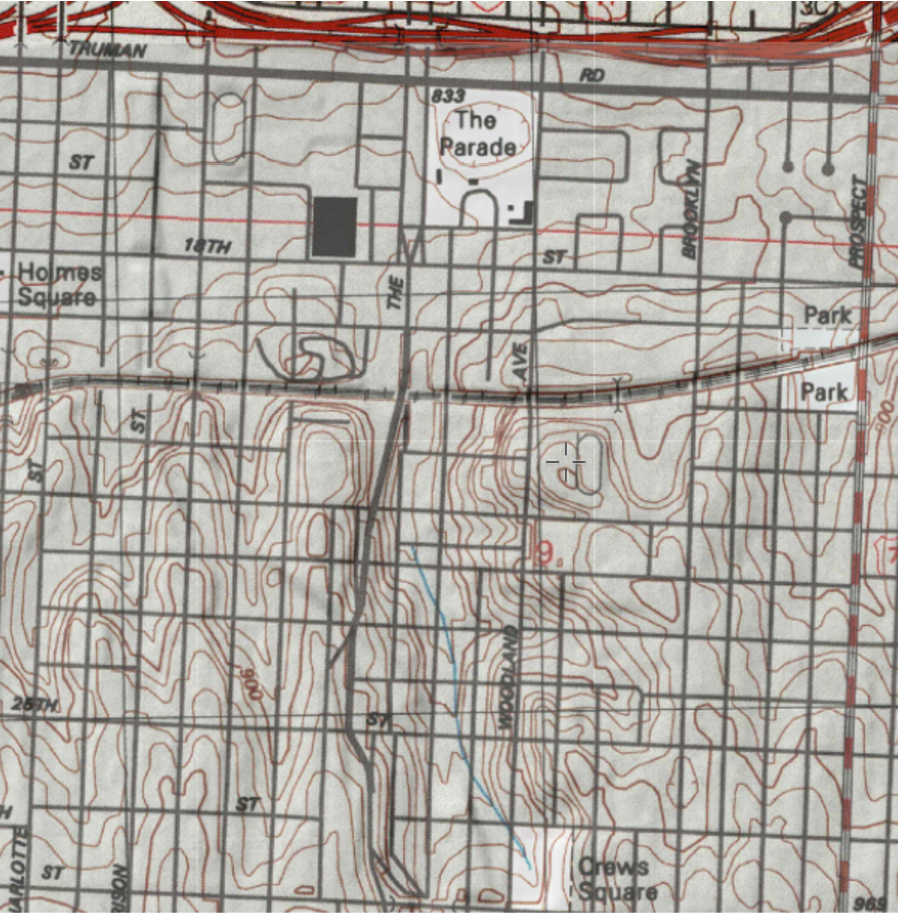
\includegraphics[width=5in]{lp_es_topo.pdf}}
\end{center}

 Lincoln Prep's commanding vista covers
a great many points north and northwest, in addition to allowing for redundant
interconnection to existing KCFN infrastructure.  Those areas obscured by the
gradients that lead to 71 Highway and the 18\textsuperscript{th} \& Vine valley are
significantly devoid of residences.  Close proximity to
existing KCFN infrastructure at 18\textsuperscript{th} \& Vine compensates adequately for the
lack of clear line of sight  between Lincoln Prep and the Parade Park Homes
residential area. \par
The areas to the south and east of the target area contain the
majority of residences in the target area. Light to moderate foliage and slight
east-west gradients there preclude one-hop access to Lincon Prep from some
locations. In order to compensate, a FreedomTower near 27\textsuperscript{th} \& Prospect
would be highly beneficial.
Finally, there is a significant outcropping of homes in the southwest corner of
the area with no visibility of either Lincoln Prep or the 27\textsuperscript{th} \& Prospect
area. To connect these homes to the network would likely require the
construction of a small FreedomTower at Wendel Phillips Academy. \par
In general, the terrain of the target area does not present a significant
obstacle, and is in many ways expedient to network construction. \par
\subsubsection{RF Environment}
The RF Environment shows heavy utilization in the 2.4GHz band, with light though
not insignificant usage in the 5GHz band. Our finding is that while appropriate
channel selection for devices will be critical, there is ample spectrum
available for use in the target geography. In order to assess spectrum health,
we conducted spot surveys at ten strategic locations. A dual-band 802.11 radio
running in monitor mode cycled through all available channels, capturing and
logging WiFi data frames. While it is highly unlikely that there are any non-WiFi
emissions of concern, any such emissions were not captured or detected using
this methodology. A statistical analysis of the resulting frame logs was conducted
by comparing the total frames captured per channel to the number of available
timing slots, weighting for the ratio of beacon frames to data frames, and
normalizing for total channel capacity. The resultant metric is a reasonable
approximation of how much data capacity is being used in each channel, and how
much remains. While some minor deviations do exist
between the individual spot surveys, the deviations are small enough that the
data pool taken as a whole is highly reflective of the spectrum usage across
the entire area. The graph below reflects the average values across all ten
survey locations: \par
\begin{center}
\fbox{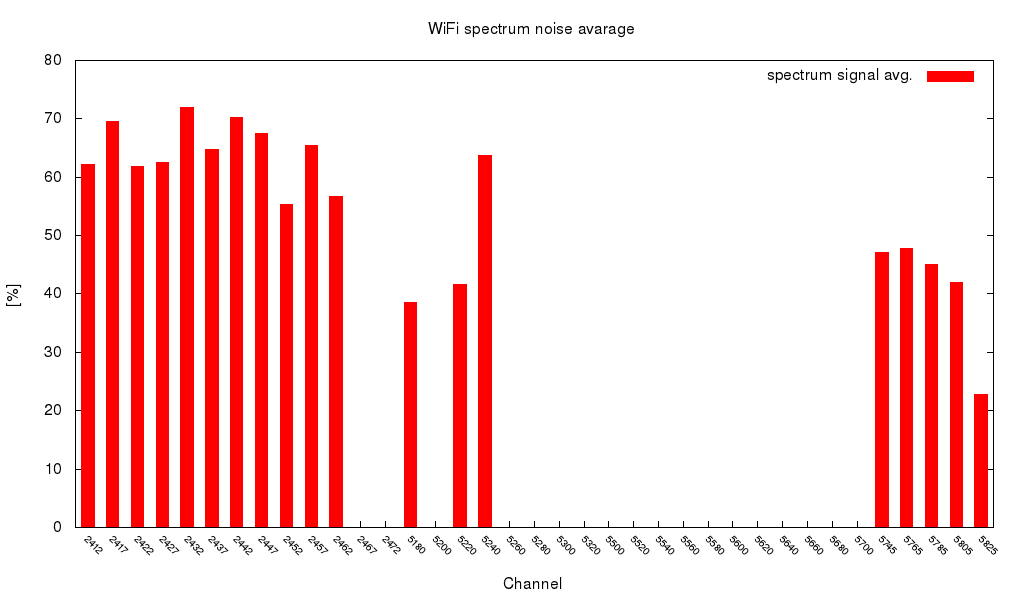
\includegraphics[width=5in]{spectrum.png}}
\end{center}
All told, this graph depicts a spectrum that is certainly utilized, but has plenty of room
in the 5GHz band. While the more popular 2.4GHz band is crowded, the fact that
it is slated for use only in Access Point deployments mitigates most of our
concern. In general, the spectrum looks more or less as expected, and aligns
well with the presuppositions of the Free Network Architecture.

\subsection{Findings}
On the basis of our survey results and prior field experience, we have devised
a proposed plan of action and associated cost estimates. These projections are intended
to serve as a starting point for collaboration, and certainly do not reflect the
only viable path towards accomplishing the stated objectives.\par

\subsubsection{Proposed Plan}
\begin{description}
\item[Phase I - Autumn 2013]
As a first phase, we recommend the construction of a FreedomTower atop Lincoln
Prep, and organization of an enrichment education opportunity for
students there. This would immediately create opportunities for block-level
organization across much of the study footprint. The LP tower would be
connected to existing KCFN infrastructure at 31\textsuperscript{st} \& Troost
and 18\textsuperscript{th}
\& Vine, and to the School District's network via an auxilliary router at
Lincoln Prep. Ideally, this tower would be constructed by student technicians
under the supervision of the Free Network Foundation and Connecting for Good. \par
As part of this first phase, it would be necessary to lay the social and
political groundwork for further growth. School administrators, student
engineers, and members of the KCFN would reach out directly to those potential
partners identified in subsequent phases, and to the community at large. \par

\item[Phase II - Winter/Spring 2014]
When the Lincoln Prep tower has been functioning for some time, and a small
corps of network volunteers has been established, additional towers should be
built to expand coverage to the rest of the study area. We have identified
Kansas City Storage, at 2431 Prospect, and Wendell Phillips Academy, at 1619 E
24\textsuperscript{th} Terrace, as ideal sites for subsequent construction. With these three
towers alone, the vast majority of targeted residential blocks would have the
ability to opt in by constructing a FreedomRelay. \par
While it certainly makes sense for the school district to fund  construction
of the network infrastructure at its facilities, and potentially to subsidize
those relays and nodes necessary to reach its students, long term success
depends on a highly distributed ownership model. As such, it will be of critical
importance that the network coalition engage in a concerted 
effort to publicly demonstrate the benefits of the network.\par

\item[Phase III - Summer 2014 \& Beyond]
After the network backbone has been constructed in Phases I and II, the
focus should shift entirely to community stakeholdership and organic growth.
Those students and community members that have been trained as network
technicians will maintain existing infrastructure and facilitate the
construction of new networks on a voluntary or commercial basis. \par
At this point, the network would be well situated for expansion south and east,
towards those areas of the city with the greatest need for affordable access.
Future partners could include libraries, community centers, neighborhood
associations, additional schools, and all those who recognize the opportunity
for mutual benefit inherent in the free network model.\par
\end{description}

\subsubsection{Costs \& Figures}
While the community-driven model has its definite strengths, it can also make it
difficult to give precise estimates of cost. Below we present
those costs that can be immediately quantified, as well as figures intended to
give an idea of the total investment that would be required to achieve desired
levels of coverage. Bear in mind that this investment would be, in a sense,
`crowdsourced', and that any particular stakeholder would be liable only for a
modest fraction of the total cost. \par

The construction of a FreedomTower at Lincoln Prep would
have the following hard costs:
\begin{center}
\begin{tabular}{|p{5cm}|l|l|l|}
\hline
Item & Q'ty Req'd & Unit Cost & Total Cost \\ \hline
Ubiquiti ToughCable & 2000ft & \$.22/ft & \$220 \\ \hline
Ubiquiti ToughConnectors & 20 & \$.53 & \$10.60 \\ \hline
Ubiquiti ToughSwitch-8 & 1 & \$188 & \$188 \\ \hline
Ubiquiti Rocket M5 & 5 & \$85 & \$425 \\ \hline
Ubiquiti RocketDish 5G30 & 2 & \$150 & \$300 \\ \hline
Ubiquiti Sector 5G19-120 & 3 & \$140 & \$420 \\ \hline
3-Gang Cluster Mount & 1 & \$131 & \$131 \\ \hline
Alix 2D13 Router & 1 & \$139 & \$139 \\ \hline
1.75" EMT Conduit & 10' & \$1.35/ft & \$13.50 \\ \hline
VMP FRM-200 Mount & 1 & \$80 & \$80 \\ \hline
18"x8"x8" Cinder Block & 6 & \$1.60 & \$9.60 \\ \hline
Total Hardware & - & - & \$1,935.70 \\ \hline
\end{tabular}
\end{center}
Subsequent towers would have slightly lower costs. Build funders would retain
complete ownership of all hardware, in accordance with the Network Commons
License.\par

The labor for all builds should come from volunteer and student technicians working
under the supervision of Connecting for Good engineers. Such a volunteer corps
would also constitute the first tier of operational support for the network.
While Connecting for Good would maintain responsibility for keeping the
infrastructure up and running in Phases I \& II, this responsibility should be
transferred to community operators in Phase III. In exchange for supervising
these builds, and taking responsibility for maintaining the Tower infrastructure
in Phases I \& II, Connecting for Good would require compensation of \$10,000. \par

While expanding an existing network is a well-documented process, integration
with KCPS's existing network infrastructure will take a significant engineering
effort. For this work, and for educational consultancy during Phases I \& II of
the build process, the Free Network Foundation would require compensation of
\$10,000.

While it is impossible to tell in advance, we
estimate that to connect every home and business in
the area would require 3 FreedomTowers, with 30 FreedomRelays per tower, and 40
FreedomNodes per relay, for a total cost of ~\$230,000. In actuality, it is
highly unlikely that total coverage will be required, and the costs should be
far less. Keep in mind that the vast majority of this investment would come from
the community, at a cost of ~\$25/person for the above. Even this estimate is conservative, as
it doesn't take into account the role of businesses and associations, which are
the most likely entities to sponsor neighborhood and block-level hardware. \par

A small upfront investment in backbone infrastructure and education, if properly
channeled, has the potential to enable massive, distributed community
improvement. Investing  primarily in know-how, rather than in infrastructure
itself, sets the stage for commercial opportunity, and long-term sustainability.

